\chapter{Diversity}
\label{cp:Diversity}

\section{Species Richness}
A total of 77 bird species were recorded during the study period. This includes birds from 40 different families.\\
Out of 331 regular land bird species found in Sri Lanka, this is roughly 23.2\%.

\begin{figure}[!htpb]
    \centering
    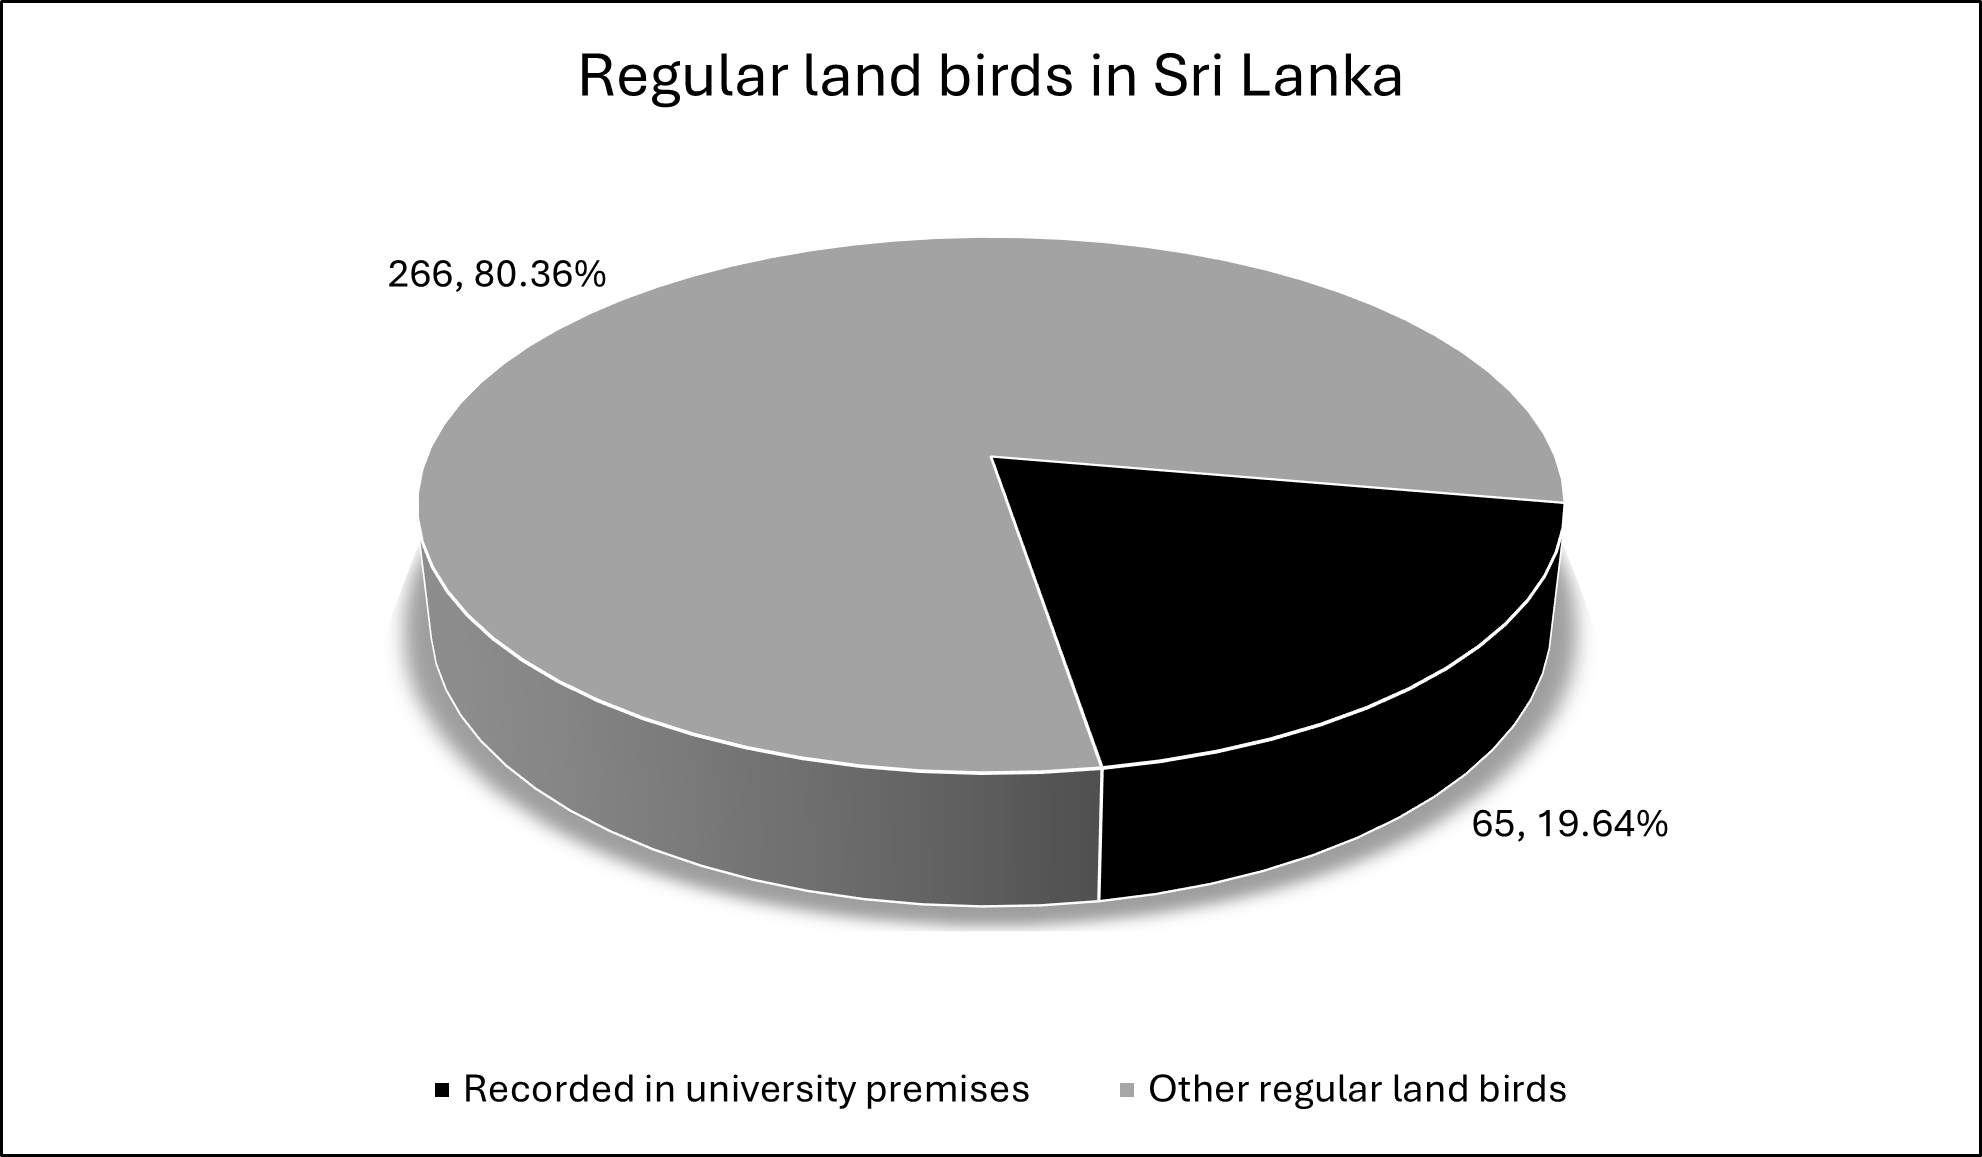
\includegraphics[width=\linewidth]{Figures/pieChart1.png}
    \caption[]{Pie Chart showing the recorded number of regular land birds species in the university out of the regular land birds recorded in Sri Lanka.}
    \label{fig:figure-01}
\end{figure}


\section{Conservation Significance}
The checklist includes some Vulnerable species and a Critically Endangered species. Five out of the 77 birds are endemic to Sri Lanka, including,
\begin{itemize}
    \item Ceylon Swallow (\textit{Cecropis hyperythra})
\item Crimson-fronted Barbet (\textit{Psilopogon rubricapillus})
\item Sri Lanka Green Pigeon (\textit{Treron pompadora}).
\item Lesser Sri Lanka Flameback (\textit{Dinopium psarodes}) and
 \item Sri Lanka Hanging Parrot (\textit{Loriculus beryllinus}).
\end{itemize}
% \nameref{cp:citations} (referred to as \autoref{cp:citations}).

\section{Rarity of Species}
While some of the species recorded are very common in university premises and some others are relatively rare, there were even some species that was recorded only once during the period of study.
\begin{itemize}
    \item Indian Golden Oriole (\textit{Oriolus kundoo})
    \item Painted Stork (\textit{Mycteria leucocephala})
    \item Changeable Hawk Eagle (\textit{Nisaetus cirrhatus})
    \item Black-Winged Stilt (\textit{Himantopus himantopus})
    \item Indian Robin (\textit{Saxicoloides fulicatus})
    \item Striated Heron (\textit{Butorides striata})
\end{itemize}
falls under this category.
